\graphicspath{{chapters/13/}}
\chapter{Construction of phylogenetic trees}
\emph{A method based on \textbf{mutation distances} as estimated from cytochrome \textit{c} sequences is of general applicability (1967)}

\section{What are phylogenetic trees}
They are graphs made up of nodes, which represent the taxonomic units and from branches that join the nodes, representing the distances between the two.
\\
Topology is defined as the general structure of a tree. If to the branches evolutionary distance is not given, we have a cladogram (I), otherwise we have a filogram (II) and with time a dendogram (III).
\\
Trees without root do not foresee evolutionary meanings in time terms and describe simply the relationships between sequences. Trees with root they accept the hypothesis as true of the molecular clock and the nodes they are in a specific
temporal order.
\begin{figure}[H]
		\centering
		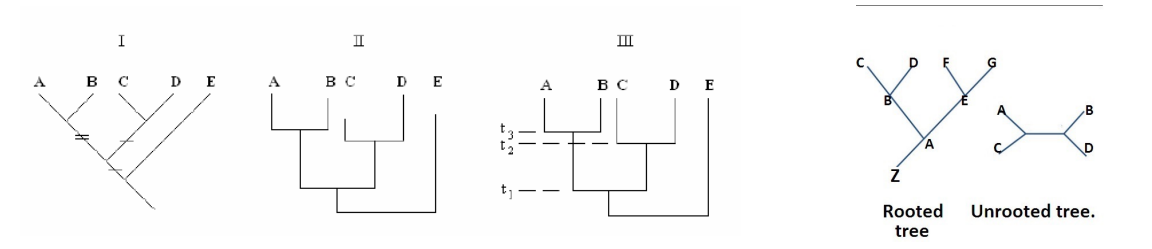
\includegraphics[width=0.9\textwidth]{grams.png}
		\caption{Topologies of phylogenetic trees}
		\label{fig:1}
	\end{figure}

\section{Introduction}
Some methods to constructs phylogenetic trees were developed before the one that will be discussed here, like studies of the degree of interspecific hybridization of DNA, number of amino acid replacements between homologous proteins, etc.
These methods are not satisfactory, because:
\begin{itemize}
\item i) the portion of the genome examined was often very resticted
\item ii) Low accuracy in the mutation distance between the genes examined
\item iii) no adequate mathematical treatment of large datasets
\end{itemize}

To tackle especially points ii) and iii), a new method is hereby proposed and the validity of the results is carried out with the construction of a tree considering only cytochrome \textit{c}, for much much information is available.
Even just considering one gene, the resulting tree is much similar to the phylogenetic tree constructed directly from biological data.

\subsection{Ancenstral genes, Orthologs and Paralogs}
Among homologous genes, one has to distinguish \textbf{orthologous} from \textbf{paralogous} sequences. Orthologs are \textbf{homologous} genes in different species that diverged from a single \textbf{ancestral gene} after a speciation event and paralogs are homologous genes that originate from the intragenomic duplication of an ancestral gene.

\subsection{Proteins or nucleic acids?}
For molecular phylogeny it is preferable to use nucleotide sequences.
In phylogeny both are used, but it is necessary to fix some key aspects that define the different action ranges of the two:
\begin{itemize}
\item Protein sequences
	\begin{itemize}
	\item need 20x20 replacement matrices, very complex to deal with
	\item are the expression of coding regions only
	\item identical amino acids can be the expression of multiple codons
	\end{itemize}

\item Nucleotide sequences
	\begin{itemize}
	\item they can be described with 4x4 matrices.
	\item can be extracted from non-coding genomic sequences, therefore with higher variation
	\item they have no degeneration or redundancy.
\end{itemize}

\end{itemize}

\section{Determining the mutation distance}
The mutation distance between two cytochromes is defined here as the minimal number of nucleotides that would need to be altered in order for one cytochrome to code for the other. This distance is determined by making pair wise comparison of homologous amino acids. For each pair a mutation value is taken from a pre-defined table, which gives the minimum number of nucleotide changes required to convert the coding from one amino acid to the other. 
\\
For each possible pairing of cytochromes, the 110 mutation values found are summed to obtain the minimal mutation distance. 
The basic approach tot he construction of the tree is illustrated in figure \ref{fig:1}, which shows three hypothetical proteins, A, B and C, and their mutation distances. There are two fundamental problems: 

\begin{itemize}
\item Which pair to join first? As a first approximation, one solves it by simply choosing the pair with the smallest mutation distance, which in this case is A and B, with a distance of 24. A and B are shown connected at the lower apex. 
\item What are the lengths of legs \textit{a, b} and \textit{c}? One notes that the distance from A to C, 28, is 4 less than the distance form B to C. Meaning, there must have bee at least 4 countable mutations in the descent of B from the lower apex than in the descent of A.
\end{itemize}

\begin{figure}[H]
		\centering
		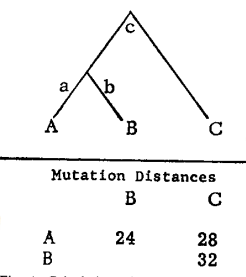
\includegraphics[width=0.4\textwidth]{1.png}
		\caption{Calculation of observed mutation distances. The upper apex represents a hypothetical ancestral organism that divided into two descending lines, one of which subsequently also divided. Thus we have three present-day species, A, B, C. The number of observable mutations that have occurred since the A and B lines of descent diverged are represented respectively by \textit{a} end \textit{b}. The number of mutations that separate the lower apex and C is represented by \textit{c}. The sums of $a+b, a+c, b+c$ then are the mutation distances of the three species as currently observed.}
		\label{fig:1}
	\end{figure}


When information from more than three protein is utilized, the basic procedure is the same, except that initially each protein is assigned to its own subset. One then simply joins two subsets to create a single, more comprehensive subset, and the process is repeated until all proteins are members of  a single subset. 
A phylogenetic tree is but a grphical representaion of the order in which the subsets were joined. 
\\
In the case of this study, they started with 20 subsets, each subset consisting of a single cytochrome \textit{c} amino acid sequence. One arbitrarily accepts, from among all the possible pairings examined, that assigned of protein subsets to sets A, B and C which provides the lowest average mutation distance from A to B. The leg lengths are then recorded. Henceforth the proteins of A and B so joined are treated as a single subset, and the entire procedure described in the preceding paragraph is repeated.  Thus the number of proteins($N$) is reduced by 1 at each cycle. The tree will be produced after $N-1$ joinings. 

\subsection{Genetic distances}
\emph{From slides, lec 13}
\\
For the phylogenetic distinction of two sequences, it is necessary to know how much they diverge. We therefore need an objective parameter and a calculable, defined genetic distance. 
For conserved nucleic acids, the number of percentage substitutions observed after multiple alignments

\begin{equation}
d = \frac{n. replacements}{length}
\end{equation}

For less conserved nucleic acids the \textit{d} is corrected with the Jukes-Cantor formula:

\begin{equation}
d'= -\frac{3}{4}log(1- \frac{4}{3} d)
\end{equation}

For proteins, aligned with a replacement matrix, it is often used the approximated formula:

\begin{equation}
d =  \frac{(Sobs - Srand)}{(Smax -Srand}
\end{equation}

With Sobs the score of the alignment, Smax average of the scores of the alignments of all proteins with themselves, Srand score expected for sequences of the same length and composition. 

\section{Testing alternative trees}
Because of the arbitrary nature of the rule by which proteins were assigned to sets A and B, the initial tree will not necessarily represent the best use of the information. The solution provided by the authors is simply to construct another tree by assigning an alternative pair of protein subsets to sets A and B whenever the mutation distance between the two subsets is not greater by some arbitrary amount than that between the members of the initial pair used in constructing the initial phylogenetic tree. 

\subsection{Standard deviation}
If the absolute difference between two such mutation distances $|(i,j)-(j,i)|$ is multiplied by $100$ and divided by (i,j), the result is the  of change from the input data. If such values are squared and the squares are summed over all values of $i < j$, the resultant sum ($\mathcal{E}$) may be used to obtain the percent "standard deviation" of the reconstructed values from the input mutation distances. The number of mutation distances summed is $N(N-1)/2$. The number is reduced by 1, divided into the sum $\mathcal{E}$ and the square root taken, the result is the percent "standard deviation". 

\section{The statistically optimal tree}
In testing phylogenetic alternatives, one is seeking to minimize the percent standard deviation.
\\
In addition to using a single gene product to discover evolutionary relationships among several species, one can similarly delineate evolutionary relationships among different genes (int he paper the gene phylogeny, from the amino acid sequence was reconstructed for human alpha, beta, gamma and delta hemoglobinn chains and whale myoglobin).
\\
A cautionary note may be derived from this. A wildly incorrect result could e easily be obtained if the presence of multiple, homologous genes were not recognized and a phylogeny were reconstructed from sequences which were coded for, say, half by genes for alpha hemoglobin chains and half by genes for beta hemoglobin chains. This results from the speciation having occurred more recently than the gene duplication which permitted the separate evolution of the alpha and beta genes.

\section{Phylogenetic relationships in trees}
\emph{From slides, lec 13}
\\ 
The systems for building trees aims to discover how the sequences are in
relation to each other: the data (the sequences themselves or distances) are used to create a system of equations that models "when" the sequences diverge (the nodes) and how extensive it is the separation separation (branches).

It starts from a theoretical tree in which the various OTUs are inserted, without giving importance to the various branches. The goal is to understand how, how much and where they fork using various criteria, not necessarily molecular.

\subsection{Fitch-Margoliash algorithm (FM)}
\begin{figure}[H]
		\centering
		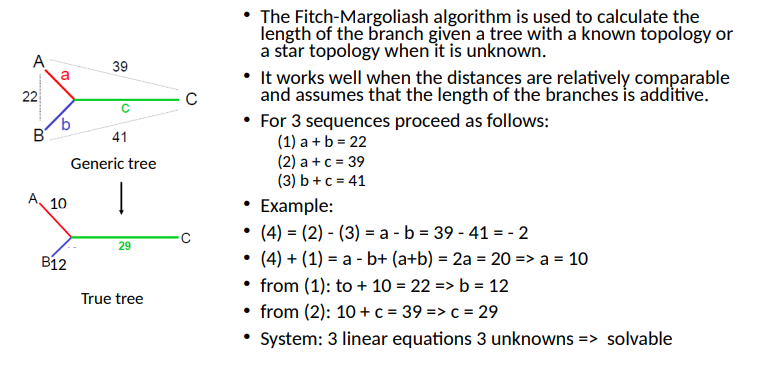
\includegraphics[width=0.8\textwidth]{ex1.png}
		\caption{}
		\label{fig:ex1}
	\end{figure}
















